\documentclass[conference]{IEEEtran}
\IEEEoverridecommandlockouts
% The preceding line is only needed to identify funding in the first footnote. If that is unneeded, please comment it out.
\usepackage{cite}
\usepackage{amsmath,amssymb,amsfonts}
\usepackage{algorithmic}
\usepackage{graphicx}
\usepackage{textcomp}
\usepackage{xcolor}
% User packages
\usepackage{hyperref}
% \usepackage[brazilian]{babel}

% Default arameters
\def\BibTeX{{\rm B\kern-.05em{\sc i\kern-.025em b}\kern-.08em
    T\kern-.1667em\lower.7ex\hbox{E}\kern-.125emX}}

% User parameters
\newcommand{\reviewUrgent}[1]{{\color{red} #1}} % This command is used for mandatory changes
\newcommand{\reviewNormal}[1]{{\color{yellow} #1}} % This command is used for a strong suggestion
\newcommand{\reviewMinor}[1]{{\color{green} #1}} % This command is used for minor changes suggestion

\begin{document}

\title{Conference Paper Title}

\author{\IEEEauthorblockN{Brewton Morais}
\IEEEauthorblockA{\textit{DETI} \\
\textit{Universidade Federal do Ceará}\\
Fortaleza, Brazil \\
\href{mailto:brewtonlmorais@gmail.com}{brewtonlmorais@gmail.com}}
\and
\IEEEauthorblockN{Lucas Abdalah}
\IEEEauthorblockA{\textit{DETI} \\
\textit{Universidade Federal do Ceará}\\
Fortaleza, Brazil \\
\href{mailto:lucasabdalah@alu.ufc.br}{lucasabdalah@alu.ufc.br}}
}

\maketitle

\begin{abstract}
An analysis of classification models was done for a set of data with informations related
to the request and approvals for research and academic activities. Using MATLAB 2022a, 
we trained different classification models, statistical and decision trees, such as 
Logistic Regression, KNN, LDA, CART, etc, making use of their respective confusion 
matrix as the results demonstrations. One of the goals these tests is to investigate if 
there are linear relationship between the provided predictors of the data base, in 
order to optimize the model that could be used by an university or a governamental 
instituion. Finally, we perform a comparison of the results and of the decision making
about which model we understand to be the most efficient to the problem.  

\end{abstract}

\begin{IEEEkeywords}
classification model, logistic regression, grand application, KNN.
\end{IEEEkeywords}

\section{Introduction}



\reviewNormal{This command is used for a strong suggestion.}

\reviewMinor{This command is used for minor changes suggestion.}

Classification models are a class of mathematical models constantly used in problems of
assimilating observations of certain events to certain categories that define the problem.
Nowadays, these models are considered tools of fundamental importance in the construction 
of Deep Learning and Machine Learning algorithms. To begin, it's important to evidence 
the main existing difference between this new class of models and the class of 
regression models which is the prediction of a qualitative variable instead of a quantitative
one. This new class of tools present various practical applications, such as the 
development of a detection spam filter for emails based on the sender and on the content
of the message, the development of classification techniques of a cell belonging to tumors, 
as beningn or malignant and on the development of a model of credit release for financing.

In addition to these pure classification models applications, there are mixed applications 
techniques that combine Data Mining techniques with some other types of models to perform
a prediction. Some examples of models that use Data Mining practices to improve their 
results are addressed by Sidropoulos \reviewNormal{Add reference}, such as Web Mining/Search 
tensor models and Brain Data Analysis. 

Meanwhile, in the work developed in this paper, some of the most used routines in the
development of classification models were approached, such as Support Vector Machine (SVM),
K-Neirest Neighbors (KNN) \cite{Patrick} and Classification and Regression Tree (CART), to train and 
test a funding model that will separate observations into one of two available groups:
Positive Founding and Negative Founding.

KNN (\ref{KNN}) uses the concept of proximity or distance to make 
classifications of an individual data point, based on the other points surrounding it. Simply,
we assume that data points close to one another up until some threshold belong to the same class.
SVM (\ref{SVM}) is a set of supervised learning used for classification. One of its
advantages is its efficience in high dimensional spaces, even when the number of 
predictors is greater than the number of samples. However, unlike Logistic Regression,
it doesn't directly provides probability values. Decision Trees (\ref{Decision Tree})
are a non-parametric method for classification and regression. In short, the way it 
works is by efficiently learning decision rules based on the data set, that will
predict the final output as being of a class, or another. It's important to state 
that this method is quite efficient with $N>2$ classes. Intuitevely, it simply checks 
some conditions one after another, which are the decision rules, and link the response of those 
conditions to a certain class at the final step. One good advantage of this method is that it 
doesn't require much data pre-processing, so it's not necessary to create dummy variables or 
to normalize the data.  


\section{Method}

\subsection{Data set}

The data used for the construction of the predictive models consists of 8708 samples
of different requests for funding from universities around the world, to finance research,
with the outcome being the success or failure of the request. The data set contains samples
from the years 2005 to 2008, with a total of 1882 predictors (independent variables). 
6633 samples from 2005 to 2007 and 1552 from 2008 were used for model training, and the 
remaining 518 samples from 2008 were used for testing the obtained model. Predictors can be 
separeted between continuous, such as the number of successes and failures passed by the 
"chief investigator", and categorical ones, such as the monetary value of the grant, 
divided into 17 groups of increasing amounts, and the month of application.

\subsection{Pre-processing}

Initially, the first step is verifying the data skewness, in case there is a strong 
tendence to the left or to the right, an adequate transformation would be applied in order to 
remove the skewness. The next step is to scale and center the data around the mean. It's 
done so since different predictors can have different scales, and if they're not normalized,
models sensitive to the variance would be affected negatively, making it biased to those
predictors with the highest values. 

Then, what we should do is to verify which predictors have actual importance to the model 
construction, that is, which of them have a stronger say for the final prediction. We can 
study this by analysing their correlation. Those with a correlation larger than 0.99, with
zero variance or sparse, that is, that have lots of zero values as data, were removed.

Then, the final approach is to verify the linearity of the predictors together with the output. 
This step is essential, and the reason for this is, once we have analysed this aspect, we can
infer if using a linear model is the adequate way of resolving this problem. For example, 
if there are too much predictos with non-linear relationship with the final output, it makes no 
sense to insist in linear prediction models.

\subsection{Cross-Validation}

Cross-validation consists in a validation technique used to validate the model with the
test set, usually taking into account the model flexibility and the mean squared error (MSE).
Shortly, it divides the data set into $k$ distinct subsets of size as equal as 
possible. From these groups, one of them is put aside to be used as validation set,
while the model is trained based on the remaining $k-1$ subsets. Once the model is trained,
the first removed subset is used as validation as previously stated. Then, the removed 
subset is restored to the principal set, and the following subset is put aside to 
perform the same procedure until all of the $k$ subgroups are all used as validation set. 
This approach improves the model capability of generalization, once it's trained with 
all the data at dispose, it also makes the error estimation more robust.

This strategy generally serves to indicate which models have a better prediction capability
on the test set, since it enables the comparison between the error levels and the variance
generated.

It's important to state that if a $k$ is chosen such as it's too small, e.g, $k=2$ 
(two subgroups) or too large ($k=$sample size), we are going to have, respectively, a 
strongly biased model because we let a lot of data outside the training step, and a potential
overfitting issue due the high model complexity, ocurring the model to have a high variance.
Thus, to mitigate both of the effects, normally $k=5,10$ is employed, since they present
an acceptable level of bias and variance.

\section{Model validation performance}

One of the most used metrics to measure the performance a classification model is the
Receiver Operating Characteristic curve (ROC) and the Area Under the Curve (AUC) \reviewNormal{correct initials?}.
 The ROC curve is traced in a graphic with the positive ratio in the y-axis and the negative
ratio in the x-axis, and each point of the curve is computed varying the classification
limiar. Decreasing this limiar makes the model classify more items as positive, increasing
the true positive and false positive. Increasing this limiar, causes the inverse
effect.

After calculating the ROC curve we can find the area under it. The area under the ROC curve
represents how well the model divides the two classes, as close the AUC value is from 1, 
better the model. However, this kind of analysis shouldn't be applied alone to validate
 a model's performance, since there is an information loss in the construction of the 
 graphic. Then, the dispersion table, which contains in its principal diagonal the number
 of true positives and true negatives, and in its secondary diagnoal the number of 
 false positives and false negatives, becomes an interesting analysis complement to the 
 ROC curve.

 \section{Linear Methods}
\subsection{Logistic Regression (LR)}
It is statistical model used to determine the probability of an event. Therefora, its values 
are probabilities, which belong to the $(0,1)$ interval. 
The model is defined as:

\begin{equation}
   p(X) = \cfrac{e^{\beta_0 + \beta_1X}}{1+e^{\beta_0 + \beta_1X}} \hspace{0.15cm}, \hspace{0.35cm} 0\leq p(X) \leq 1 \label{eq1}
\end{equation}

This logistic model will aways produce a S-shaped curve, regardless of the value of $X$, 
getting a relatively precise prediction. After some mathematical astuces, it's possible 
to come up with the following equations that model the method.

\begin{equation}
    \cfrac{p(X)}{1-p(X)} = e^{\beta_0+\beta_1X} \label{eq2}
\end{equation}

\begin{equation}
    \log \left(\cfrac{p(X)}{1-p(X)}\right) = \beta_0+\beta_1X \label{eq3}
\end{equation}

The right term of \eqref{eq2} is called Odds, then the right term of \eqref{eq3} is 
called log-odds or logistic. The Odds ratio represents the effects of predictor X, on the
likelihood that an event will happen.

To adjust the model's parameters would be necessary to use
the Maximum-Likelihood technique to perform an estimation of them. However, it's also possible
to make use of the Least Squares for the adjust, as well as in the case of the 
coefficients in a linear regression.

\reviewUrgent{Put Table 1 here}

% \begin{table}[htbp]
%     \caption{LR Test}
%     \begin{center}
%     \begin{tabular}{|c|c|c|c|c|}
%     \hline
%     \cline{1-5}
%     \textbf{Positive}& 148 & 41 & 78.38\% & 21.7\% \\
%     \cline{1-5} 
%     \textbf{Negative} & 43 & 286 & 86.9\% & 13.1\% \\
%     \hline
%      & \textbf{Positive} & \textbf{Negative} & & & \\
%     \hline
%     \end{tabular}
%     \label{LR Test}
%     \end{center}
% \end{table}

\subsection{Linear Discriminant Analysis}

Instead of directly estimating $P(Y|X)$, a model with the following characteristics will 
be developed:

\begin{itemize}
    \item Modeling the distribution of predictors of X separately in each class Y.
    \item Baye's Theorem to estimate $P(Y = K|X = x)$.
    \item Normal distribution to describe each class.
\end{itemize}

Following from these informations, we initiate the model's development directly from the 
Baye's Theorem:

\begin{equation}
    P(Y=k|X=x) = p_k(X) \label{eq4}
\end{equation}

\begin{equation}
    p_k(X) = \cfrac{P(X=x|Y=k)P(Y = k)}{P(X=x)} \label{eq5}
\end{equation}

\begin{equation}
    p_k(X) = \cfrac{\pi_k f_k(x)}{\sum^{K}_{l=1}\pi_lf_l(x)} \label{eq6}
\end{equation}

Where $f_k(x)$ represents the probability density function (pdf) of the r.a X of 
an observation belonging to class K. Thus, instead of directly computing $p_k(X)$ it's 
possible to simply estimate $\pi_k(X)$ and $f_k(X)$. Then, assuming that the number of 
predictors is unitary, we can make some affirmations about the form of $f_k(x)$ in order
to move on with the LDA method:

\begin{equation}
    f_k(x) = \cfrac{1}{\sqrt{2\pi\sigma^2_k}}e^{\cfrac{-(x-\mu_k)^2}{2\sigma^2_k}} \label{eq7}
\end{equation}

Besides, we assume $\sigma_1^2=...=\sigma_k^2$. Therefore, it's possible to write $p_k(X)$ 
as the following:

\begin{equation}
    p_k(X) = \cfrac{\pi_k \cfrac{1}{\sqrt{2\pi\sigma^2_k}}e^{\cfrac{-(x-\mu_k)^2}{2\sigma^2_k}}}{\sum^K_{l=1}\cfrac{1}{\sqrt{2\pi\sigma^2_l}}e^{\cfrac{-(x-\mu_l)^2}{2\sigma^2_l}}} \label{eq8}
\end{equation}

After some algebraic manipulations, it's possible to conclude that classifying one
observation to a given class is equivalent to classify one observation to a given class 
such that the the linear discriminant function $\sigma_k(x)$ is larger:

\begin{equation}
    \sigma_x = x\cfrac{\mu_x}{\sigma^2} - \cfrac{u_k^2}{2\sigma^2} + \log(\pi_k) \label{eq9}
\end{equation}

However, in practical situations, it's not always possible to know the parameter's values,
then LDA approximates the Bayes classifier by the following expressions:

\begin{equation}
    \hat{\mu_k} = \frac{1}{n_k} \sum^K_{i = k} x_i \label{eq10}
\end{equation}

\begin{equation}
    \hat{\sigma^2} = \frac{1}{n-K} \sum^K_{i = k} \sum^K_{i = k} (x_i-\hat{\mu_k})^2 \label{eq11}
\end{equation}

\begin{equation}
    \pi_k = \frac{n_k}{n}\label{eq12}
\end{equation}


\reviewUrgent{Put Table 2 here}


\section{Non-Linear Methods}

\subsection{Quadratic Discriminant Analysis (QDA)}

The QDA method is a non-linear variant of the LDA. The main difference between QDA and LDA
lies in the fact that the covariance matrix of each class is different onr from another:

\begin{equation}
    X \sim  \mathcal{N}(u_k, \textstyle \sum_k)\label{eq13}
\end{equation}

The discriminant function for this method is, after some algebraic astuces:

\begin{equation}
    \sigma_k(x) = -\frac{1}{2}(x-\mu_k)^T\sum^{-1}_k(x-\mu_k) - \frac{1}{2}\log \lvert\sum_k\rvert +\log(\pi_k) \label{eq14}
\end{equation}

\begin{equation}
\begin{aligned}
    \sigma_k(x) = {} 
    & -\frac{1}{2}x^T\sum^{-1}_kx + x^T\sum^{-1}_k\mu_k -  \frac{1}{2}\mu_k^T\sum^{-1}_k\mu_k - \\ 
    & - \frac{1}{2}\log \lvert\sum_k\rvert +\log(\pi_k) \label{eq15}
\end{aligned}
\end{equation}

Thus, the QDA may be summarized as a way of computing $\sum_k$, $\mu_k$ and $\pi_k$ 
in order to use the discriminant equation in the classification of a X observation into a class
in which the discriminant has the larger absolute value.  

Therefore, the QDA method is mainly recommended when there is a sufficiently large data set
so the statements about the variance don't be a need or when it is not possible to 
sustain the statement abour the unicity of the covariance matrix. Hence, differently 
of the LDA method, the decision region of QDA is described by a non-linear curve. 

\subsection{K-Nearest Neighbors (KNN)}
\label{KNN}
Generally in practice, informations about the conditional distribution of Y given X 
are not available. That being the case, the Baye's classification method works only as 
a comparison tool to other more easily applicable practices. From this need of developing 
methods that don't rely on previous statements about the form of the boundary of decision,
the KNN routine takes place.

Shortly, KNN is a model such that its result is define by a "voting", where each "vote", 
is the amount of K samples closer of elements surrounding the analysed point which belongs
to a certain class. The class having the larger amount of points, or votes, wins. 

Something important to define in KNN methods is how the distances would be measured between
the samples, given that the classifiers are not in lenght units. Starting from this premise,
considering the vector $\textbf{x} = [p_{x_1}, ..., p_{x_n}]$, and $\textbf{n} = [p_{n_1}, ..., p_{n_n}]$, 
where $\textbf{x}$ the vector that represents the sample to be classified and $\textbf{v}$
is the neighbor vector to be computed the distance. Therefore, the most traditional way 
of computing the distance, is using the Euclidian Distance:

\begin{equation}
    d = \sqrt{\langle (x-v), (x-v)\rangle} \label{eq16}
\end{equation}

Of course there are a lot of other ways of computing the distance between the samples. 
In the training phase, the best results were obtained by using the Spearman Distance computation
method, where the vector measures are taken into account and represented by $\overline{\cdot}$, and it is 
given as: 

\begin{equation}
    d = 1 - \cfrac{\langle (x-\overline{x}), (v - \overline{v})\rangle}{\langle \sqrt{\langle (x-\overline{x}), (v - \overline{v})\rangle}, \sqrt{\langle (x-\overline{x}), (v - \overline{v})\rangle}\rangle}
\end{equation}

This distance was used in a test with 50 neighbors, together with the use of weights that
considered the inverse of the square distance, and in order to not harm its performance, the data weren't standardized, being the second more well succeeded than
the previous and also than the pure distance. However, by means of reference, the results 
depicted in table 3 were computed without weights and with Euclidian Distance.

Since KNN does not classify the samples by probabilities, one way of making it possible is to 
make the probabilities related to votes of each sample. This is done by the following 
equation. which defines the conditional probabilities, with $K \in \mathbb{Z}^{+}$ referent 
to the neighbors and an observation $x_0$ in a set $N_0$ and the function $I(\cdot)$
returns 1 if the sample $y_i \neq j$ and 0 otherwise.

\begin{equation}
    P(Y = j|X = x_0) = \frac{1}{K} \sum_{i \in N_0} I(y_i = j) 
\end{equation}

Finally, to conclude the KNN algorithm the Baye's Rule must be applied to classify the 
observations $x_0$ into the class with the highest probability of occurence. It's 
interesing to notice that for $K$ close to 1, the decision boundary is extremely 
flexible, corresponding to a classifier with low polarization (low bias) and with 
high variance. Meanwhile, for a large K, the exact opposite is true.

\reviewUrgent{Add table 3} 

\reviewUrgent{Add table 4}


\subsection{Support Vector Machine (SVM)}
\label{SVM}
In its simplest form, SVM separates points of two different classes using a single
hyperplane with the Statistical Learning Technique, both developed by Vapnik (1995) and (1998) \reviewUrgent{add reference}.
In the more complex versions, an hyperplane is built in $\mathbb{R}^n$, for a $n>2$, for 
the class split, the increase of $n$ leaves the problem with a non-linear solution. In general,
it's used the expression in \eqref{eq19} to define the decision boundary, i.e, the hyperplane
for the separation of classes in $\mathbb{R}^2$.

\begin{equation}
    D(u)=\beta_0 + \sum_{j=1}^P \beta_j\mu_j = \beta_0+\sum_{i = 1}^ny_i\alpha_ix_i'u, \hspace{0.5cm} \alpha_i \geq 0 \label{eq19}
\end{equation}

\reviewUrgent{Add table 5}

\subsection{Decision Tree}
\label{Decision Tree}
This method is quite robust and it comes from a simple principle: divide the approach
into levels and attributes to build a cost function. To facilitate the visualization,
it's interesing to use a binary tree. In general, the approach is given by decision levels,
and for each level an attribute is chosen such that it better splits a data set 
according to the class.

\reviewUrgent{Add figure 1}

For each new chosen attribute, new branches are created for the values present in the list
of all possible attributes values. The way this is implemented depends on the algorithm
used. In our work, we opted for the CART algorithm. The attributes choice in this model
is made based on the Gini Criterion, which deals with node impurity, defined in \reviewUrgent{Add Reference here}
by Breiman (1984) as:

\begin{equation}
    \sum_{j \neq i} p(i|t)p(j|t) \label{eq20}
\end{equation}

In short, we can assume that the criterion associates an object randomly selected from a 
node to the class $i$ with probability $p(i|t)$. Meanwhile, $p(j|t)$ refers to the 
estimated error probability that the item belongs to class $j$, such that the $p(j|t)$
is the Gini Indice.

The Gini Criterion works with one class at a time, aiming to separate the more frequent 
class objects from the remaining objects in each test. 

The well detailed explanation it's really important, since one of the factors that may 
influence the precision and the time consumed to classify is the number of nodes present.
Look at the tables (6) and (7) \reviewNormal{cite tables}, there are represented the results
with trees of 10 and 100 nodes, respectively. The number of nodes didn't have much influence
in the confusion matrix.

\reviewUrgent{Add table 6}

\reviewUrgent{Add table 7}

\section{Results and Discussion}

\subsection{Training results}

During the training phase of all the models proposed, we applied the cross-validation 
with $k=10$ subgroups, allowing protection against overfitting. To verify the results
on the training set, we look at figure (2) and table (8). From the figure, we can 
conclude that non-linear methods, such as SVM and the Decision Trees with 100 nodes, 
have better performance when compared to simpler methods, such as Decision Trees with 10 
nodes and Linear Methods.

However, this pattern does not hold on the test set, since the linear models obtained 
a quite good generalization capacity, making them as efficient as the non-linear models.

\subsection{Conclusion}

Among the test results obtained, there were no relevant differences between the results 
of the models, with an exception of KNN, which had the worst result, but still, not bad. 
A probable cause of this performance of KNN, it's that there are probably a data skewness, 
since the "nature" of KNN, will preferentially classify the data located at the side 
containing more elements, the evidence to it is in the table (4), since there is a 
good classification performance in one of the classes, what suggests that this class 
is more numerous, distorcing the remaining class classification.

This similarity on the results between linear and non-linear methods, means that 
the classes "success" and "failure" are linearly or approximately linearly separable. 
Therefore, it favors the choice of simplest models of less computational cost. 
According to the generated test, the best model was the Quadratic SVM. On the other hand,
that performance was only superior in one hit in comparison with the LDA model. The latter
can be trained with a lot less time and generate equivalent results. 

Like KNN, other models had more considerable errors in one of the classes. The Logistic
Regression had a correct rate smaller in the class "success" than in the "failure" class.
Meanwhile, in the decision trees algorithms, the situation is inverted.  The algorithms 
presenting a better trade-off in the class classification were the LDA and the 
Quadratic SVM, with a difference around two percentual points between the correct 
classification rates.

Having raised these considerations, we conclude that the model with the best
trade-off is the LDA, as its results with respect to corrected classified rates and 
time of training are better than the results of other traditional methods. Its 
corrected classified rate was not discrepant between classes, besides being equiparable 
to the non-linear method with the best performance on the test set. The only caution would 
be if it was necessary to often remodel the methods as more data were to be added.
To this specific situation, the Decision Tree with 10 nodes would be recommended, in order to be 
more agile in the training phase with a large data set. 
% \subsection{Equations}
% Number equations consecutively. To make your 
% equations more compact, you may use the solidus (~/~), the exp function, or 
% appropriate exponents. Italicize Roman symbols for quantities and variables, 
% but not Greek symbols. Use a long dash rather than a hyphen for a minus 
% sign. Punctuate equations with commas or periods when they are part of a 
% sentence, as in:
% \begin{equation}
% a+b=\gamma\label{eq}
% \end{equation}

% Be sure that the 
% symbols in your equation have been defined before or immediately following 
% the equation. Use ``\eqref{eq}'', not ``Eq.~\eqref{eq}'' or ``equation \eqref{eq}'', except at 
% the beginning of a sentence: ``Equation \eqref{eq} is . . .''

% \subsection{\LaTeX-Specific Advice}

% Please use ``soft'' (e.g., \verb|\eqref{Eq}|) cross references instead
% of ``hard'' references (e.g., \verb|(1)|). That will make it possible
% to combine sections, add equations, or change the order of figures or
% citations without having to go through the file line by line.

% Please don't use the \verb|{eqnarray}| equation environment. Use
% \verb|{align}| or \verb|{IEEEeqnarray}| instead. The \verb|{eqnarray}|
% environment leaves unsightly spaces around relation symbols.

% Please note that the \verb|{subequations}| environment in {\LaTeX}
% will increment the main equation counter even when there are no
% equation numbers displayed. If you forget that, you might write an
% article in which the equation numbers skip from (17) to (20), causing
% the copy editors to wonder if you've discovered a new method of
% counting.

% {\BibTeX} does not work by magic. It doesn't get the bibliographic
% data from thin air but from .bib files. If you use {\BibTeX} to produce a
% bibliography you must send the .bib files. 

% {\LaTeX} can't read your mind. If you assign the same label to a
% subsubsection and a table, you might find that Table I has been cross
% referenced as Table IV-B3. 

% {\LaTeX} does not have precognitive abilities. If you put a
% \verb|\label| command before the command that updates the counter it's
% supposed to be using, the label will pick up the last counter to be
% cross referenced instead. In particular, a \verb|\label| command
% should not go before the caption of a figure or a table.

% Do not use \verb|\nonumber| inside the \verb|{array}| environment. It
% will not stop equation numbers inside \verb|{array}| (there won't be
% any anyway) and it might stop a wanted equation number in the
% surrounding equation.

% \subsection{Some Common Mistakes}\label{SCM}
% \begin{itemize}
% \item The word ``data'' is plural, not singular.
% \item The subscript for the permeability of vacuum $\mu_{0}$, and other common scientific constants, is zero with subscript formatting, not a lowercase letter ``o''.
% \item In American English, commas, semicolons, periods, question and exclamation marks are located within quotation marks only when a complete thought or name is cited, such as a title or full quotation. When quotation marks are used, instead of a bold or italic typeface, to highlight a word or phrase, punctuation should appear outside of the quotation marks. A parenthetical phrase or statement at the end of a sentence is punctuated outside of the closing parenthesis (like this). (A parenthetical sentence is punctuated within the parentheses.)
% \item A graph within a graph is an ``inset'', not an ``insert''. The word alternatively is preferred to the word ``alternately'' (unless you really mean something that alternates).
% \item Do not use the word ``essentially'' to mean ``approximately'' or ``effectively''.
% \item In your paper title, if the words ``that uses'' can accurately replace the word ``using'', capitalize the ``u''; if not, keep using lower-cased.
% \item Be aware of the different meanings of the homophones ``affect'' and ``effect'', ``complement'' and ``compliment'', ``discreet'' and ``discrete'', ``principal'' and ``principle''.
% \item Do not confuse ``imply'' and ``infer''.
% \item The prefix ``non'' is not a word; it should be joined to the word it modifies, usually without a hyphen.
% \item There is no period after the ``et'' in the Latin abbreviation ``et al.''.
% \item The abbreviation ``i.e.'' means ``that is'', and the abbreviation ``e.g.'' means ``for example''.
% \end{itemize}
% An excellent style manual for science writers is \cite{b6}.

% \subsection{Authors and Affiliations}
% \textbf{The class file is designed for, but not limited to, six authors.} A 
% minimum of one author is required for all conference articles. Author names 
% should be listed starting from left to right and then moving down to the 
% next line. This is the author sequence that will be used in future citations 
% and by indexing services. Names should not be listed in columns nor group by 
% affiliation. Please keep your affiliations as succinct as possible (for 
% example, do not differentiate among departments of the same organization).

% \subsection{Identify the Headings}
% Headings, or heads, are organizational devices that guide the reader through 
% your paper. There are two types: component heads and text heads.

% Component heads identify the different components of your paper and are not 
% topically subordinate to each other. Examples include Acknowledgments and 
% References and, for these, the correct style to use is ``Heading 5''. Use 
% ``figure caption'' for your Figure captions, and ``table head'' for your 
% table title. Run-in heads, such as ``Abstract'', will require you to apply a 
% style (in this case, italic) in addition to the style provided by the drop 
% down menu to differentiate the head from the text.

% Text heads organize the topics on a relational, hierarchical basis. For 
% example, the paper title is the primary text head because all subsequent 
% material relates and elaborates on this one topic. If there are two or more 
% sub-topics, the next level head (uppercase Roman numerals) should be used 
% and, conversely, if there are not at least two sub-topics, then no subheads 
% should be introduced.

% \subsection{Figures and Tables}
% \paragraph{Positioning Figures and Tables} Place figures and tables at the top and 
% bottom of columns. Avoid placing them in the middle of columns. Large 
% figures and tables may span across both columns. Figure captions should be 
% below the figures; table heads should appear above the tables. Insert 
% figures and tables after they are cited in the text. Use the abbreviation 
% ``Fig.~\ref{fig}'', even at the beginning of a sentence.

% \begin{table}[htbp]
% \caption{Table Type Styles}
% \begin{center}
% \begin{tabular}{|c|c|c|c|}
% \hline
% \textbf{Table}&\multicolumn{3}{|c|}{\textbf{Table Column Head}} \\
% \cline{2-4} 
% \textbf{Head} & \textbf{\textit{Table column subhead}}& \textbf{\textit{Subhead}}& \textbf{\textit{Subhead}} \\
% \hline
% copy& More table copy$^{\mathrm{a}}$& &  \\
% \hline
% \multicolumn{4}{l}{$^{\mathrm{a}}$Sample of a Table footnote.}
% \end{tabular}
% \label{tab1}
% \end{center}
% \end{table}

% \begin{figure}[htbp]
% \centerline{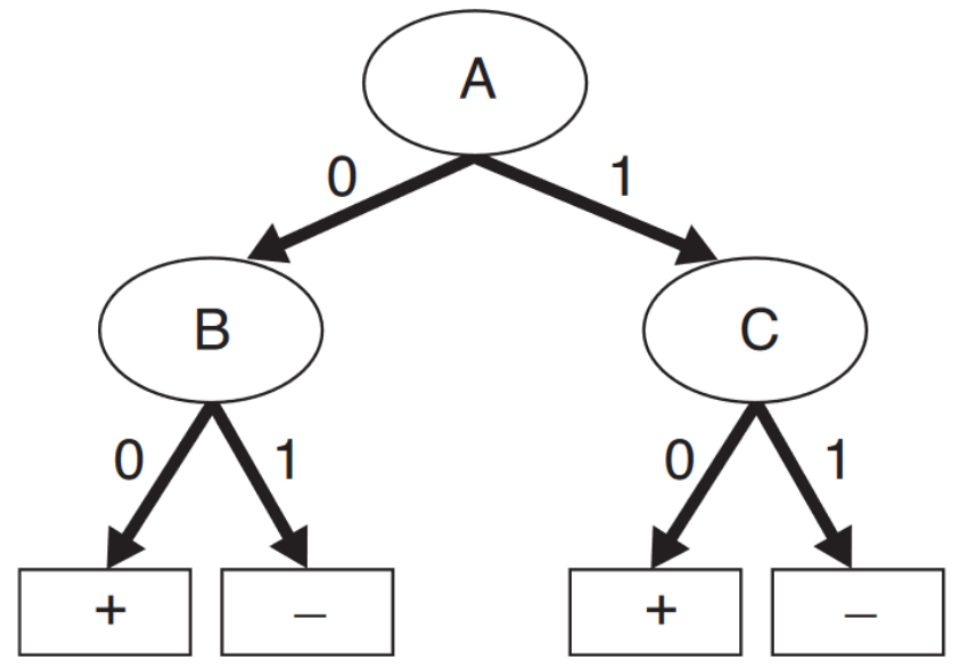
\includegraphics{fig1.png}}
% \caption{Example of a figure caption.}
% \label{fig}
% \end{figure}

% Figure Labels: Use 8 point Times New Roman for Figure labels. Use words 
% rather than symbols or abbreviations when writing Figure axis labels to 
% avoid confusing the reader. As an example, write the quantity 
% ``Magnetization'', or ``Magnetization, M'', not just ``M''. If including 
% units in the label, present them within parentheses. Do not label axes only 
% with units. In the example, write ``Magnetization (A/m)'' or ``Magnetization 
% \{A[m(1)]\}'', not just ``A/m''. Do not label axes with a ratio of 
% quantities and units. For example, write ``Temperature (K)'', not 
% ``Temperature/K''.

% \section*{Acknowledgment}

% The preferred spelling of the word ``acknowledgment'' in America is without 
% an ``e'' after the ``g''. Avoid the stilted expression ``one of us (R. B. 
% G.) thanks $\ldots$''. Instead, try ``R. B. G. thanks$\ldots$''. Put sponsor 
% acknowledgments in the unnumbered footnote on the first page.

% \section*{References}

% Please number citations consecutively within brackets \cite{b1}. The 
% sentence punctuation follows the bracket \cite{b2}. Refer simply to the reference 
% number, as in \cite{b3}---do not use ``Ref. \cite{b3}'' or ``reference \cite{b3}'' except at 
% the beginning of a sentence: ``Reference \cite{b3} was the first $\ldots$''

% Number footnotes separately in superscripts. Place the actual footnote at 
% the bottom of the column in which it was cited. Do not put footnotes in the 
% abstract or reference list. Use letters for table footnotes.

% Unless there are six authors or more give all authors' names; do not use 
% ``et al.''. Papers that have not been published, even if they have been 
% submitted for publication, should be cited as ``unpublished'' \cite{b4}. Papers 
% that have been accepted for publication should be cited as ``in press'' \cite{b5}. 
% Capitalize only the first word in a paper title, except for proper nouns and 
% element symbols.

% For papers published in translation journals, please give the English 
% citation first, followed by the original foreign-language citation \cite{b6}.

\bibliographystyle{ieeetran}
\bibliography{refs}

\vspace{12pt}
\color{red}
IEEE conference templates contain guidance text for composing and formatting conference papers. Please ensure that all template text is removed from your conference paper prior to submission to the conference. Failure to remove the template text from your paper may result in your paper not being published.

\end{document}
